\section{\green{Methods}}

I am following the assumption that we don't start from a blank slate but from some initial concepts, here operationalised as primitives, fundamental program components. These initial primitives comprise a minimal domain-specific lanugage (DSL) and can be composed into more complex programs, which represent the causal structure generating the observations we perceive. As such, an agent learns its own DSL, which in terms of a language of thought is analogous to inferring a mental grammar and using it to learn new concepts.



\subsection{\green{FlowCoder}}

We have seen how a probabilistic program synthesis algorithm looks like and what it can achieve [change this sentence]. 
Moreover, we have learnt that sampling might be a good alternative to enumerative search and that GFlowNets are a method to implement a generative model and sampler. Additionally, we have learnt that LLMs which use the Transformer architecture learn statistical regularities that go beyond syntax into the semantic realm. In the following I will show how I combine all these concepts to arrive at my own model \textrm{FlowCoder} \footnote{Code available at \url{https://github.com/R1704/master_thesis}}.


Why do we do it?
\begin{enumerate}
    \item First, I want to investigate whether GFlowNet is an adequate strategy within the realm of program synthesis. Can a GFlowNet be trained to be a good sampler?
    \item Another reason for using GFNs over DreamCoder or other methods is that we build programs sequentially. This makes the method more dynamic and gives us more control. For example we can do inferences about intermediate latent variables, train from partial states, etc. [should this be here or in discussion?]
    \item We want to embed programs. This gives us an additional semantic layer. [compare with neural pcfg, and other approaches and criticisms of dreamcoder]
    \item I want to learn the whole probabilitiy dist to a task, not just the MAP.
\end{enumerate}






Research Questions: what do we want to find out
\begin{enumerate}
    \item 
\end{enumerate} 



\subsubsection{\green{DeepSynth Framework}}

Both in DreamCoder and DeepSynth, programs are represented as abstract syntax trees (ASTs). An AST is a tree representation of the syntactic structure of the program, with nodes representing operations or primitives and edges representing their compositional relationships. In order to avoid predicting variables, deBruijn indexing is used, which is a technique to represent bound variables in a way that avoids naming conflicts and simplifies variable substitution [source]. Named variables are replaced with numeric indices representing the number of enclosing $\lambda$ abstractions that bind the variable. See figure \ref{fig:AST} for a visualisation of an AST using deBruijn indexing.

\begin{figure}[H]
    \centering
    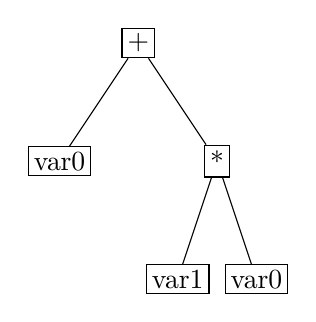
\begin{tikzpicture}
        [
        every node/.style={draw, inner sep=2pt},
        level distance=1.5cm,
        level 1/.style={sibling distance=2cm},
        level 2/.style={sibling distance=1cm}
        ]
        
        \node {+}
        child {
            node {var0}
        }
        child {
            node {*}
            child {
            node {var1}
            }
            child {
            node {var0}
            }
        };
    \end{tikzpicture}
    \caption{An example of an abstract syntax tree (AST) using deBruijn indexing. This translates to \texttt{var0 + var1 * var0}.}
    \label{fig:AST}
\end{figure}

Here, an initial DSL along with suitable syntactic constraints compile into a context-free grammar (CFG), which defines the possible structures of programs within its DSL. A CFG consists of a set of production rules that describe how to generate strings from a set of non-terminal and terminal symbols. It's "context-free" because the production rules are applied regardless of the surrounding symbols.
In DeepSynth, a prediction model is used to predict weights for a probabilistic CFG (PCFG), extending the CFG by associating probabilities with the production rules. This allows the grammar to not only generate the syntactic structure of a program but also to represent beliefs about the relative plausibility or frequency of different structures \footnote{See appendix \ref{app:cfg} for a formalisation of CFGs and PCFGs.}. This is similar to DreamCoder's transition matrix which is outputted by the recognition model. The PCFG guides the search and inference process towards more likely programs. DreamCoder however, does not specifically use a PCFG. Both frameworks employ a typed $\lambda$-calculus, hence there are restrictions on program arguments, etc. (syntactical constraints). DreamCoder performs type inference during program generation. To spare computational cost, DeepSynth constructs the CFG beforehand which in turn increases the size of the CFG.

\subsubsection{\green{GFlowNet}}\label{sec:gflownet}
In the following I will give a detailed explanation of GFlowNet
\todo[inline]{should this be here or in intro? Explain why we explain this. 1. to show how the algorithm works, 2. to show how we deal with the marginalisation term}

GFlowNets create a directed acyclic graph (DAG) over the state space, where vertices correspond to states or partial samples and edges denote transitions or adding a component to a partial sample, in which the edges carry a flow from source to targets \cite{bengio2023gflownet, bengio_flow_2021}.
\todo[inline]{show diagram of DAG and talk about the causality requirement! (In the methods section we explain what we do and why we do it.)}
In GFlowNets, the "flow" in the network corresponds to the process by which the network constructs a sample, which can be thought of as a path in a graph where nodes are partial samples, and edges correspond to adding a component to the partial sample.
The core training objective for a GFlowNet is to satisfy the flow matching constraint. The idea is to ensure that the flow into any state (a partially constructed sample) should match the flow out of it, given the reward associated with complete samples. The flow here refers to the expected transitions into or out of a state under the model's stochastic policy. 
Formally, a state \( s \) represents a partial object a certain stage in the generative process. A trajectory \( \tau \) is a sequence of states \( s_0, s_1, ..., s_T \) that the model traverses from an initial state \( s_0 \) to a terminal state \( s_T \), where the target structure is complete.
A trajectory \( \tau \) is formed by a sequence of actions \( a_1, a_2, ..., a_T \), where each action \( a_t \) transitions the model from state \( s_{t-1} \) to state \( s_t \). The sequence of actions is governed by a policy \( \pi \), which defines the probability of choosing a particular action given the current state.
The flow \( F(\tau) \) of a trajectory \( \tau \) is defined as the product of the probabilities of each transition along the trajectory, multiplied by the reward \( R(s_T) \) of the terminal state, normalized by a partition function \( Z \).

\begin{equation} \label{eq:flow}
    F(\tau) = \frac{R(s_T)}{Z} \prod_{t=0}^{T-1} \pi_\theta(s_{t+1} | s_{t})
\end{equation}

The partition function \( Z \) ensures that the sum of flows over all possible trajectories equals one, effectively normalising the distribution. Since we don't know \( Z \), we can estimate it by parameterizing it as \( Z_{\theta} \).
The flow matching constraint enforces that for any given non-terminal state \( s \), the total flow into \( s \) must equal the total flow out of \( s \):

\begin{equation} \label{eq:flow_match}
    F(\tau) = F(\tau')
\end{equation}

where \( F(\tau') \) is the reverse trajectory.
We can utilize this property to create a suitable loss function to train the GFlowNet \cite{malkin_trajectory_2022}. Combining equations \ref{eq:flow} and \ref{eq:flow_match} gives us:

\begin{equation}
    \frac{R(s_T)}{Z_\theta} \prod_{t=0}^{T-1} \pi_\theta(s_{t+1} | s_{t}) = \frac{R(s_0)}{Z_\theta} \prod_{t=0}^{T-1} \beta_\theta(s_{t} | s_{t+1})
\end{equation}

Here \( \beta \) is the backward policy, predicting parent states. 
The initial state \(s_0\) has the total flow and no reward, we can rewrite it and get:

\begin{equation}
    Z_{\theta} \prod_{t=0}^{T-1} \pi_\theta(s_{t+1} | s_{t}) = R(s_T) \prod_{t=0}^{T-1} \beta_\theta(s_{t} | s_{t+1})
\end{equation}

We can now take the log on both sides:

\begin{equation}
    \log \left(Z_{\theta} \prod_{t=0}^{T-1} \pi_\theta(s_{t+1} | s_{t})\right) = \log \left(R(s_T) \prod_{t=0}^{T-1} \beta_\theta(s_{t} | s_{t+1})\right)
\end{equation}

This can be rearranged to:

\begin{equation}
    \log Z_\theta + \sum_{t=0}^{T-1} \log \pi_\theta(s_{t+1}|s_{t}) = \log R(s_T) + \sum_{t=0}^{T-1} \log \beta_\theta(s_{t}|s_{t+1})
\end{equation}

The trajectory balance loss is the squared difference:

\begin{equation}
    \mathcal{L}_{TB} = \left(\log Z_\theta + \sum_{i=0}^{T-1} \log \pi_\theta(s_{t+1}|s_{t}) - \log R(s_T) - \sum_{t=0}^{T-1} \log \beta_\theta(s_{t}|s_{t+1})\right)^2
\end{equation}

In order to mitigate the computational [cost], I am embedding all rules rather than primitives \todo[inline]{this is explained in a later section}, such that each rule is unique. Thus, every predicted node (rule) has exactly one parent, in other words, I am essentially linearising the tree. Therefore, $\beta$ will always be $1$ and can be disregarded from the equation.
Moreover, since we are solving tasks \( x \in X \), we have a conditional reward distribution $R(s_T|x)$, as well as a conditional forward policy $\pi_\theta(s_T|x)$ and partition function $Z_\theta(x)$.
This gives us the final loss:

\begin{equation}\label{form:TB}
     \mathcal{L}_{TB} = \left(\log Z_\theta(x) + \sum_{t=0}^{T} \log \pi_\theta(s_{t+1}|s_{t}, x) - \log R(s_T \vert x)\right)^2
\end{equation}     



% Formally, the computational model is as follows:
% input: tasks x in X, DSL, syntactic constraints, reward function, hyperparameters alpha, beta, epsilon, generative model, GFN

% output: trained generative model, trained recognition model, programs solving tasks X


% \subsubsection{\orange{Compositional Latent Variable Model}}
% Finetuning our fomalisation, we can specify that our goal is to construct programs $z \in \mathcal{Z}$ where $z$ can be nested. We can therefore see it as a compositional latent variable model as described in \cite{hu_gflownet-em_2023}. 
% Given a set of observations \( X \), the marginal likelihood or evidence is:
% \begin{equation}\label{form:evidence}
% p(x) = \sum_z p_\theta (x|z) p_\theta(z)
% \end{equation}

% We can formalise the optimisation challenge as finding the parameters \( \theta \) that maximize the data's log-likelihood:
% \begin{equation} %\label{form:bayes}
%     \mathcal{L} = \log \prod_{i=1}^{T} p(x_i) = \sum_{i=1}^{T} \log \sum_{z} p_\theta(x_i|z) p_\theta(z)
% \end{equation}

% \todo[inline]{is this correct? is the optimisation challenge not over phi and theta and X?}

% The full algorithm is described in the pseudocode: \ref{alg:flowcoder}. 

\todo[inline]{We need to formalise the overall objective}

\subsubsection{\green{Expectation-Maximisation}}
Hu et al. introduce a GFlowNet-EM which utilises Expectation-Maximisation in order to deal with the difficult problem of joint optimisation \cite{hu_gflownet-em_2023} \footnote{See \url{https://github.com/GFNOrg/GFlowNet-EM/} for the accompanying code.}.
The core principle of Expectation-Maximisation (EM) involves an iterative two-step process: the Expectation (E) step computes an expectation of the log-likelihood evaluated using the current estimate for the parameters, and the Maximisation (M) step, computes parameters maximizing the expected log-likelihood found in the E-step. The GFlowNet version is slightly different and we separate the parameterisation.
In the E-step the recognition model is optimised, i.e. the forward policy of the GFlowNet that is proportional to the posterior.
Here, empirical data as well as a trajectory is sampled and the trajectory balance loss is used to update the parameters of the forward policy $\pi_\phi(z|x)$, i.e. $\nabla_\phi \mathcal{L}_{TB}$.
In the M-step also empirical data and a trajectory is sampled but only the reward is used to update the parameters of the generative model $p_\theta(x \vert z) p_\theta(z)$.




\subsubsection{\green{Sleep}}
As sleep has been proven to be a crucial element of the models success, I am utilising it too. 
\begin{description}
    \item[Replay] In Replay, I am training the forward policy on previously correctly solved task-program pairs $(x, z)$, using the trajectory to guide the model to the correct solution and optimising on the forward logits. Here $x$ is sampled from the empirical distribution and $z$ is sampled from the forward policy $\pi_\phi$. Additionally, I apply a sleep weight $\gamma$ to strengthen the gradient. Formally:
    \begin{equation}
        \nabla_\phi\mathcal{L}_{\text{Replay}} = \mathbb{E}_{x \sim X, z \sim \pi_\phi(z|x)} \left[ - \gamma \cdot \log \pi_\phi(\tau \vert x, z) \right]
    \end{equation}
    If a correct solution has been found during the E-step, I immediately let the model train on these trajectories of correct solutions so as to consolidate these.
After the E-step I again train the model on a set (in the mathematical sense, meaning no duplicates) of all the correct solutions, so that it doesn't forget solutions to other tasks.
Replay is applied stochastically, given the hyperparameter \texttt{replay\_prob}.
    \item[Fantasy] During Fantasy I train the model on programs constructed during the E-step and run tasks from the empirical distribution through those programs to create correct task-program pairs $(x, z)$. Then, similarly to the methodology of Replay, I train the model on these pairs. Formally:

    \begin{equation}
        \nabla_\phi\mathcal{L}_{\text{Fantasy}} = \mathbb{E}_{x \sim X, z \sim \pi_\phi(z|x)} \left[ - \gamma \cdot \log \pi_\phi(\tau \vert x, z) \right]
    \end{equation}
    Fantasy is also applied stochastically, given the hyperparameter \texttt{fantasy\_prob}. 
    \todo[inline]{filtering out programs that produce None, constants, etc. }
\end{description}


\subsubsection{\green{Optimisation Techniques}}\label{sec:optim}
Hu et al. propose a few optimisation techniques which proved to be useful \cite{hu_gflownet-em_2023}. I adapted these techniques and will describe them in the following.
\begin{description}
    \item[E-step Loss Thresholding] Rather than training the GFlowNet to a loss of zero after each M-step, we can apply a linearly decreasing moving average loss $\delta$ as a threshold to trigger the M-step using the hyperparameter $\alpha$, to save computational cost. Here I use the recursive formula:

    \begin{equation}\label{eq:threshold}
        \delta = \alpha \cdot \mathcal{L}_{TB} + (1 - \alpha) \cdot \delta
    \end{equation}
    \item[Exploration] Since we want to find many modes in the E-step and want to avoid getting stuck in local optima, several exploration techniques can be employed.
    The hyperparameter $\{\beta \vert \beta \in \mathbb{R}_{[0, 1]} \}$  can be used to exponentiate the forward policy: $ \pi_\theta(s_{t+1}|s_t)^\beta $.
    Moreover, $\epsilon$-uniform sampling can be used to the deter the model from repeating known routes by mixing the predicted logits with a uniform distribution. $\epsilon$ is chosen to be $\{\epsilon \vert \epsilon \in \mathbb{R}_{[0, 1]} \}$.
\end{description}


\begin{algorithm}[H]
    \caption{FlowCoder}
    \begin{algorithmic}[1]
    \Require Data $X$, generative model with parameters $\theta$, forward policy with parameters $\phi$, optimization and exploration hyperparameters, threshold $\alpha$
    \Repeat
        \State Sample $x \sim X$
        \State Sample $z \sim \pi_\phi(z|x)$
        \State \textbf{E-step}: gradient update on $\phi$ with $\nabla_\phi \mathcal{L}_{TB}$
        \If{$r \in (0, 1) < \texttt{replay\_prob}$}
            \State gradient update on $\phi$ with $\nabla_\phi\mathcal{L}_{\text{Replay}}$
        \EndIf
        \If{$r \in (0, 1) < \texttt{fantasy\_prob}$}
            \State gradient update on $\phi$ with $\nabla_\phi\mathcal{L}_{\text{Fantasy}}$
        \EndIf
        \If{$\mathcal{L} < \alpha$}
            \State Sample $z \sim \pi_\phi(z|x)$
            \State \textbf{M-step}: gradient update on $\theta$ with $\nabla_\theta[-\log p_\theta(x|z)p_\theta(z)]$
        \EndIf
    \Until{some convergence condition}
    \end{algorithmic}
    \label{alg:flowcoder}
    \end{algorithm}







\subsection{\green{Parameterisation}}


% All modules are written using PyTorch \cite{NEURIPS2019_9015}.

\subsubsection{\orange{Generative Model}}
In section \ref{sec:llm} we have seen that the underlying mechanism of the Transformer architecture used in LLMs, is able to learn syntactic and semantic structure from its data.
Kim et al. discuss the benefit of a distributed representation of PCFGs, over the classic notion of simply assigning a scalar to each rule of the CFG to attain a PCFG  \cite{kim_compound_2019}. To that extent I will utilise the Transformer as the generative model.

A fundamental component of the Transformer is the self-attention mechanism, formalized as:

\begin{equation}
    \text{Attention}(Q, K, V) = \text{softmax}(\frac{QK^T}{\sqrt{d_k}})V
\end{equation}

This mechanism, through the query (Q), key (K), and value (V) matrices, allows the model to dynamically assign importance to different parts of the input sequence. The scaling factor $\sqrt{d_k}$ normalizes the dot product, aiding in stabilizing gradients during training.

Moreover, the Transformer employs Multi-Head Attention, enabling the model to concurrently process information from different representation subspaces, enhancing its capability to capture diverse features. 

In this project, I am using the standard PyTorch implementation [source + see parameters in table ].

The generative model initializes with two crucial components: the IOEncoder and the StateEncoder. The IOEncoder processes input-output pairs, converting them into continuous vector representations, while the StateEncoder deals with encoding the CFG rules. See sections \ref{sec:ioencoder} and \ref{sec:ruleencoder}.
Positional Encoding is applied to the output of both encoders. This step is vital as it adds information about the sequence order to the model, allowing the Transformer to interpret the sequence data effectively.
GFlowNet employs two types of masks: padding masks for IO sequences and square subsequent masks for state sequences. These masks are crucial for handling variable-length sequences and maintaining the integrity of the data through the Transformer. The padding mask ensures that the model does not process padding tokens, while the square subsequent mask prevents positions from attending to subsequent positions, maintaining the autoregressive property in the generation process.
During the forward pass, GFlowNet processes both IO and state data through their respective encoders, applies positional encoding, and then inputs them into the Transformer. The output of the Transformer is then fed into both the forward policy and partition function networks, yielding the forward logits and log $Z$, respectively.


\begin{itemize}
    \item explain that ASTs are 2D but to use a transformer we need to linearize it. We could have also used GNN, tree transformer, etc. but it has been shown that transformer learns fine. 
    \item We could embed parent, child, etc. to make ean embedding of a rule more informed. i chose not to do it to see whether its enought (discuss in limitations,e tc. )
\end{itemize}


\subsubsection{\green{Forward Policy}}
The forward policy is implemented as a Multi-Layer Perceptron (MLP) and predicts forward logits from the Transformer's output, guiding the generative process.
[adapted from Hu]
\subsubsection{\green{Partition Function}}
The partition function $Z_\theta$ serves as a normalising factor, ensuring that the probabilities generated by the model are well-calibrated and interpretable. It is implemented as a MLP layered on top of the Transformer output.
[adapted from Hu]


\subsubsection{\green{IOEncoder}} \label{sec:ioencoder}
The IOEncoder is tasked with encoding input-output (IO) pairs into continuous vector representations.
Each input-output pair is tokenized using a predefined lexicon (a list of symbols representing the possible range of inputs and outputs), which includes special tokens such as 'PAD' (padding), 'IN' (input start), and 'OUT' (output start). This tokenization is critical for distinguishing between different parts of the input-output pairs.
The tokenized input-output pairs are concatenated into a single sequence, with the 'IN' and 'OUT' tokens demarcating the transition from input to output. Padding is then applied to ensure that all sequences have the same length, aligning them to the maximum allowed size determined by \texttt{n\_examples\_max} (the maximum number of input examples that can be processed) and \texttt{size\_max} (the maximum size of elements in a list). These parameters have been adapted from \cite{fijalkow_scaling_2021}.
The padded sequences are passed through a PyTorch embedding layer, which transforms the discrete tokens into continuous vector representations. This embedding is crucial for capturing the semantic relationships between different tokens.
During the forward pass, each batch of input-output pairs is processed, encoded, and padded to the maximum sequence length found in the batch. The sequences are then aligned and stacked to form a batch tensor, which is passed through the embedding layer. Finally, the dimensions of the output tensor are transposed to align with the requirements of subsequent model components, such as the Transformer encoder.

See table \ref{table:params} for the exact parameterisation of the model.


\subsubsection{\green{RuleEncoder}}\label{sec:ruleencoder}
The RuleEncoder in the FlowCoder framework is essential for encoding the rules of a context-free grammar (CFG) into a neural network-friendly format. This process involves transforming discrete grammar rules into continuous vector representations.
The RuleEncoder begins by collecting rules, which are pairs of non-terminals and corresponding program actions, from the CFG, provided by the DeepSynth framework. This collection includes special tokens such as 'PAD' (padding), 'START' (sequence start), and 'STOP' (sequence end). Each rule is passed through a PyTorch embedding layer.
During the forward pass, batches of state sequences (each state sequence, or trajectory, representing a series of CFG rules) are processed.
To ensure uniformity across different sequences within a batch, padding is applied.


\subsubsection{\orange{Sampling Programs}}


As described in section \ref{sec:gflownet}, a program $z$ is constructed sequentially as a trajectory $\tau$. Here, I operationalise the building blocks as the CFG rules rather than the primitives. 
Of course, we dont actually have the CFG in an adequate model of cognition, but rather we infer it.
Since DeepSynth creates a larger CFG rather than doing type inference (to save computations), I have to look up which rules are allowed syntactically to mask out unallowed rules. Of course, in principle I could also let the model create syntactically incorrect programs and give them a reward of 0 at evaluation. To speed up learning, I don't do this. However, this gives us an added benefit. There are more rules than primitives which means their embeddings are more distinct which may be easier for the model to learn.

This means that we have to convert from the representation of an array of rules to an AST program representation. Luckily this can be done easily in the DeepSynth framework.


The state of each program in the batch is initialised with a 'START' token, representing the initial state of the program generation process. A frontier, implemented as a queue, is initialized for each program to manage the sequence of non-terminals that need to be expanded. This method has been adapted from DeepSynth to fit with the FlowCoder framework and mechanisms. 
Tensors are initialized to store cumulative logits and partition functions for each program, tracking the probabilistic decisions made during the generation process.
The core of the method is a loop that continues until all frontiers are empty, indicating that all programs in the batch have been fully generated. Within this loop, the model computes logits and partition functions.
As discussed in section \ref{sec:optim}, the sampling method includes an exploration mechanism, where with a probability $\epsilon$, uniform sampling is used instead of the model's logits. This exploration is crucial for introducing variability and avoiding local optima in the generation process. Additionally, tempering is applied to logits using a factor $\beta$, modulating the sharpness of the probability distribution used for sampling.
For each program in the batch, the method iteratively samples a rule based on the current non-terminal and updates the program's state and cumulative logits. This process involves creating a mask to block invalid actions, applying the mask to logits, and sampling an action (rule) based on the masked logits.
Each sampled rule is decomposed into a non-terminal and program component, updating the program's current state and expanding the frontier with the rule's arguments.
Once all frontiers are empty, the final programs are reconstructed from their compressed representations, using methods provided by DeepSynth.


\subsection{\red{credit assignment}}\label{sec:credit}


- batches, all trajectories at once or like dreamcoder, ...
discuss the variable/ non variable batching. (credit assignment.)
mode seeking. difficulty of broad and focussed modes.




\subsubsection{\green{Reward}}

In order to train the model, we need an informative reward, i.e. it should provide a gradient, as binary rewards are not informative. As such, I am using the Levenshtein edit distance, using the \texttt{Levenshtein} package \footnote{\url{https://github.com/maxbachmann/Levenshtein}} which is a measure of the similarity between two strings. Specifically, it quantifies the minimum number of single-character edits (i.e., insertions, deletions, or substitutions) required to transform one string into another. See appendix \ref{app:levenshtein} for an in depth formalisation.

Since the Levenshtein distance returns a discrete value, I normalise it over the max length of the sequences, and since there may be more than one example per task, I average it over all examples. Moreover, I apply a max reward parameter, to scale a correct solution up and give the model a stronger gradient. In my experiments I used a max reward of 10.



\subsection{\red{reward}}

\begin{itemize}
    \item Reward should be learnt (Energy based model). Where does the brain get it from?
    \item Is Levenshtein a reasonable reward? think about computational complexity (Kologorov complexity)
    \item Reward depends on tasks
\end{itemize}





Of course we cannot just use the actual program to compare it with. In deepsynth they train by using the cross entropy loss between the nueral network aoutput and an encoding of the solution program. In reality we do not have the correct solution [think about this. we do also learn from others. so its not entirely out of question.]. Instead, we can only compare the real and predicted output. However, there are a few methods we can try to turn the comparison of sequences into a reward. Since we are working with numeric list editing, ...
Another idea is to use an energy based model, which essentially is a model that learns to predict the reward. however, this increases the computational overload and was not necessary for this toy problem.








\subsection{\green{Design}}
In the following section I will elaborate on the exact training and test methods I used, including hyperparameters.
The tasks I am using are input-output relations in the list editing domain, originally from DreamCoder. These were filtered given the syntactic constraints (e.g. type, lexicon, etc.) and provided by DeepSynth. 
In their paper, Fijalkow et al. discuss that some of the tasks are impossible solve given the DSL, so I additionally filtered those out. In my experiments I end up with 95 tasks. Each task can have between 1 and 15 examples. A task is considered solved if a program solves all examples of the task. [See appendix for tasks].
The DSL is essentially a dictionary of primitive types and semantics in a typed $\lambda$-calculus, written in Python [source] (see appendix \ref{app:dsl}).
[program depth]
Table \ref{tab:synconst} describes the syntactical constraints used in the experiment and were mostly adapted from DeepSynth and DreamCoder.

\begin{table}[H]
    \centering
    \begin{tabularx}{\textwidth}{|l|l|X|}
        \hline
        \textbf{Parameter} & \textbf{Value} & \textbf{Description} \\\hline
        \texttt{type} & \texttt{list(int) $\rightarrow$ list(int)} & The input as well as the output should be a list of integers, so the CFG should reflect that, filtering rules that do not conform to that criterion. \\\hline
        \texttt{lexicon} &  $[-30, 30] \in \mathbb{Z}$ & The lexicon is a uniform distribution of integers and in the range from -30 to 30 \\\hline
        \texttt{maximum argument number} & 1 & This is the maximum number of arguments a function could have. \\\hline
        \texttt{size max} & 10 & The maximum number of values in a list \\\hline 
        \texttt{max number of examples} & 15 & The maximum number of examples per task \\\hline 
        \texttt{depth} & 3 & The maximum depth of a program AST \\\hline 
    \end{tabularx}
    \caption{Syntactical Constraints}
    \label{tab:synconst}
\end{table}

The model was trained with a random 50/50 train-test split in random order with a batch size of 4 where each task in the batch is the same. This was done to avoid a credit assignment problem but increase efficiency. Since the forward logits are summed up and averaged over for all trajectories, the model might have confused which trajectory was rewarding. See section \ref{sec:credit} for a discussion on this matter.

Furthermore, each task is trained for 5 epochs with 2.000 E-steps and 2.000 M-steps in each epoch. The moving average threshold (see equation (\ref{eq:threshold})) $\delta$ was initialised with 150 and linearly decreases using the hyperparameter $\alpha$ set to 0.3. The exploration parameters $\beta$ and $\epsilon$ were set to $0.7$ and $0.3$, respectively. The replay and fantasy probabilities were set to 0.3 and 1, respecively, both with a weight $\gamma = 10$. The learning rates for the generative model as well as for the forward policy were set to $0.0001$. During inference I let the model run for $100$ steps. Since the batch size is 4, this creates 400 programs per task. A table of all hyperparameters can be found in appendix \ref{app:hyperparams} in table \ref{tab:hyperparams}. The experiment was run on one NVIDIA Tesla T4 GPU.





\begin{table}[H]
    \centering
    \begin{tabular}{|p{5cm}|c|c|}
        \hline
        \textbf{Task} & \textbf{Input} & \textbf{Output} \\\hline
        \texttt{remove gt 2} & \texttt{[1,2,7,5,1]} & \texttt{[1,2,1]} \\\hline
        \texttt{caesar-cipher-k-modulo-n with k=5 and n=4} & \texttt{[2, 2, 0, 1, 2, 3, 3]} & \texttt{[3, 3, 1, 2, 3, 0, 0]} \\\hline
        \texttt{prepend-index-k with k=3} & \texttt{[15, 12, 9, 14, 7, 9]} & \texttt{[9, 15, 12, 9, 14, 7, 9]} \\\hline
        \texttt{add-k with k=4} & \texttt{[16, 10, 7, 12, 13, 3]} & \texttt{[20, 14, 11, 16, 17, 7]} \\\hline
        \texttt{append-k with k=2} & \texttt{[1, 5, 15]} & \texttt{[1, 5, 15, 2]} \\\hline
    \end{tabular}
    \caption{Task Examples}
    \label{tab:task_ex}
\end{table}



\begin{table}[H]
    \centering
    \begin{tabular}{|p{5cm}|c|}
        \hline
        \textbf{Task} & \textbf{Program} \\\hline
        \texttt{remove gt 2} & \texttt{(filter (gt? 3) var0)} \\\hline
        \texttt{caesar-cipher-k-modulo-n with k=5 and n=4} & \texttt{(map (mod 4) (map (+ 5) var0))} \\\hline
        \texttt{prepend-index-k with k=3} & \texttt{(cons (index 2 var0) var0)} \\\hline
        \texttt{add-k with k=4} & \texttt{(map (+ 4) var0)} \\\hline
        \texttt{append-k with k=2} & \texttt{(append 2 var0)} \\\hline
    \end{tabular}
    \caption{Examples of tasks and programs solving the tasks.}
    \label{tab:task_programs}
\end{table}
